\documentclass[../main.tex]{subfiles}

\begin{document}

Now that we have a good theoretical context of all the parts of the problem,
we will start by analyzing the resonator with a non-kinetic inductance.

\begin{figure}
\centering
\begin{circuitikz}[]
    \draw (-0.5,0) to[short]
          (0,0) to[generic, l=\(Z_0\)]
          (1.5,0) to[capacitor, l=\(C_c\)]
          (3,0) to[short]
          (6,0);
    \draw (3,0) to[L, l=\(L\)]
          (3,-2);
    \draw (4.5,0) to[capacitor, l=\(C_p\)]
          (4.5,-2);
    \draw (6,0) to[vR, l=\({R = R_{SET} \parallel R_p}\)]
          (6,-2);
    \draw (3,-2) to[short]
          (6,-2) node[ground]{};
\end{circuitikz}
\caption{Topology of the resonator that we are going to use. \(C_{p}\) and
\(R_{p}\) are a virtual capacitor and resistance used to model losses in the
circuit, while \(R_{SET}\) is the resistance of the SET in any state. That
leaves \(C_{c}\) and \(L\) as the degrees of freedom in our system.}
\label{fig:RLC}
\end{figure}

\subsection{Resonant frequency and effective impedance}
Our analysis begins with obtaining expressions for the resonant frequency and
the effective impedance of our resonator. It's easy to see that the impedance
of our resonator in figure \ref{fig:RLC} is

\begin{equation}
\label{eq:ImpParallel}
    Z = \frac{1}{j \omega C_{p} + \frac{1}{j \omega L} + \frac{1}{R}}
        + \frac{1}{j \omega C_{c}}
\end{equation}

Which after a little massaging turns into

\begin{equation}
\label{eq:ImpParallelBinomial}
    Z = \frac{\omega^2 L^2 R}{R^2(1-\omega^2C_{p}L)^2 + \omega^2 L^2} +
        j \left(
            \frac{\omega L R^2 (1-\omega^2C_{p}L)}{R^2(1-\omega^2C_{p}L)^2 + \omega^2 L^2}
            - \frac{1}{\omega C_{c}}
          \right)
\end{equation}

The resonant frequency \(\omega_{r}\) that makes \(\Im Z = 0\) is

\begin{equation}
\label{eq:ExactWr}
    \omega_{r}^2 = \frac{1}{L(C_{c} + C_{p})}
    \left(
        1 + \frac{C_{c}}{2C_{p}} - \frac{L}{2 R^2 C_{p}} \pm
        \sqrt{\left(1 + \frac{C_{c}}{2C_{p}} - \frac{L}{2 R^2 C_{p}}\right)^2
        - 1 - \frac{C_{c}}{C_{p}}}
    \right)
\end{equation}

Choosing \(C_{c}\) and \(L\) such that
\(\frac{C_{c}}{C_{p}}, \frac{L}{R^2 C_{p}} \ll 1\), leaves us with the
approximate expression for the resonant frequency

\begin{equation}
\label{eq:Wr}
\omega_{r} \approx \frac{1}{\sqrt{L (C_{c} + C_{p})}}
\end{equation}

Finally, to obtain the effective impedance we use this expression in \(\Re Z\)

\begin{equation}
\label{eq:ExactZeff}
    Z_{eff} = \Re Z(\omega_{r}) =
    \frac{\omega_{r}^2 L^2 R}{R^2(1-\omega_{r}^2C_{p}L)^2 + \omega_{r}^2 L^2}
    \approx \frac{L (C_{c} + C_{p})}{R C_{c}^2}
      \left(1 + \frac{L (C_{c} + C_{p})}{R^2 C_{c}^2}\right)^{-1}
\end{equation}

And by, again, choosing \(L\) and \(C_{c}\) such that
\(\frac{L (C_{c} + C_{p})}{R^2 C_{c}^2} \ll 1\) we arrive to our expression for
the effective impedance

\begin{equation}
\label{eq:Zeff}
    Z_{\text{eff}} \approx \frac{L (C_{c} + C_{p})}{R C_{c}^2}
\end{equation}

In future sections we will be using quite a lot of expressions obtained via
approximations in non-approximated systems, only to do more approximations
with them. Due to this, it is really important to have a clear picture of
the regimes we are working in to ensure that our results work in the
state-of-the-art technology, and that's why after each result we are going to
recontextualize our approximations.

In this case, the approximations to obtain \(\omega_{r}\) are clear and
straight forward:

\begin{gather}
    \frac{C_{c}}{C_{p}} \ll 1 \label{eq:ApproxCcWr}\\
    \frac{L}{R^2 C_{p}} \ll 1 \label{eq:ApproxLWr}
\end{gather}

But the approximation for \(Z_{eff}\) needs a little bit of extra work. If we
multiply \((C_{c} / C_{p})^2\) in both sides, it turns into

\begin{equation}
\label{eq:ProtoZeffCond}
    \frac{L}{R^2 C_{p}} \left(1 + \frac{C_{c}}{C_{p}}\right) \ll
    \left(\frac{C_{c}}{C_{p}}\right)^2
\end{equation}

And since we used equation \ref{eq:Wr} to arrive here, it must hold
the approximation \ref{eq:ApproxCcWr}, turning the previous expression into

\begin{equation}
\label{eq:ApproximationZeff}
    \frac{L}{R^2 C_{p}} \ll \left(\frac{C_{c}}{C_{p}}\right)^2
\end{equation}

While approximations \ref{eq:ApproxCcWr} and \ref{eq:ApproxLWr} impose a
\textbf{general condition} in our degrees of freedom, approximation
\ref{eq:ApproximationZeff} imposes a \textbf{relative condition} between
the previous two.

For checking that our results are correct, we can graph the modulus of the
reflection coefficient \(\Gamma\) (equation \ref{eq:ReflecCoeff}) as a function
of the voltage frequency \(\omega\). With the standard impedance for a
transmission line \(Z_{0} = 50 \unit{\ohm}\), a parasitic capacitance
\(C_{p} = 500 \unit{\fF}\) and a resistance \(R = 50\unit{\kohm}\)
(2 times the quantum of resistance), we need to choose a \(C_{c}\) and a \(L\)
such that the conditions \ref{eq:ApproxCcWr}, \ref{eq:ApproxLWr} and
\ref{eq:ApproximationZeff} are met and \(Z_{\text{eff}} = Z_{0}\). With this in
mind, we choose \(C_{c} = 100 \unit{\fF}\) and \(L = 41.67 \unit{\nH}\)
(these values are also on the ballpark of real values used in the lab 
\hl{\textbf{REFERENCE NEEDED}}), which means that we should see \(|\Gamma|\)
dip to zero at a frequency of \(1.00654 \unit{\giga\hertz}\), which is what we
see in the black line figure \ref{fig:ReflexCoeffAndPhase}.


\begin{figure}[t]
\centering
\begin{subfigure}[T]{.5\textwidth}
  \centering
  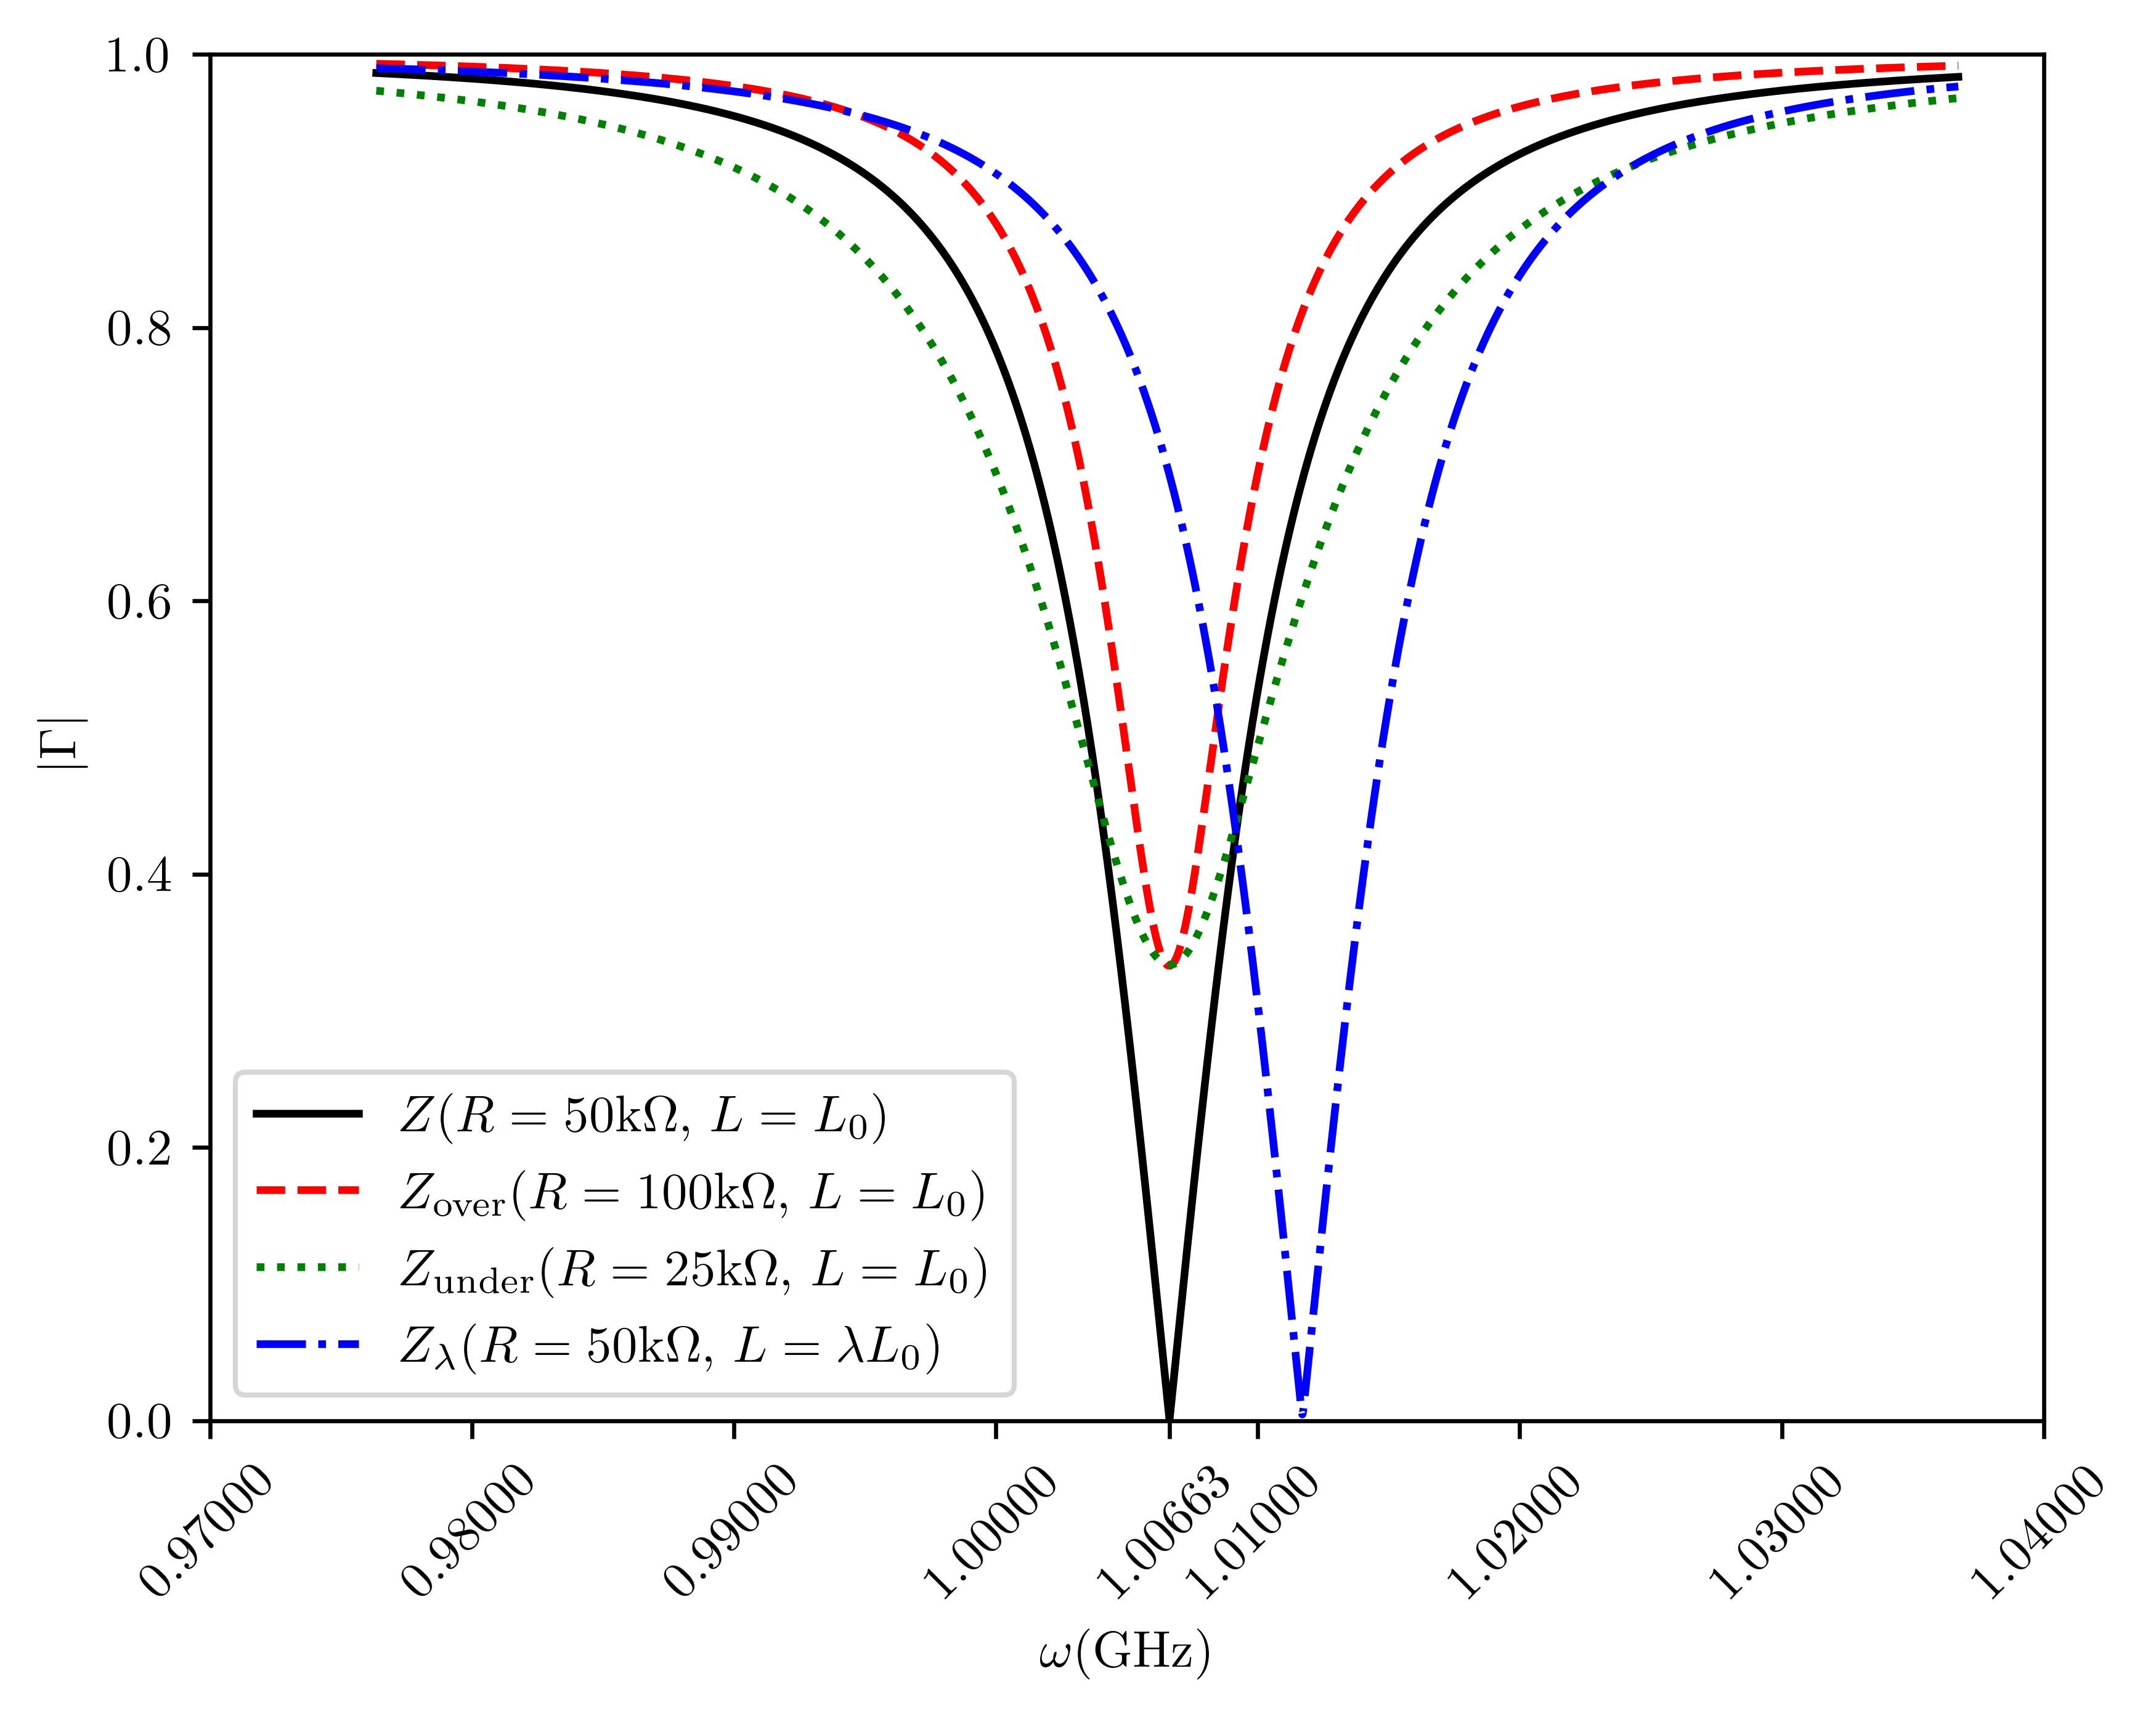
\includegraphics[width=\linewidth]{RLCParallel/ReflecCoeff.png}
\end{subfigure}%
\begin{subfigure}[T]{.5\textwidth}
  \centering
  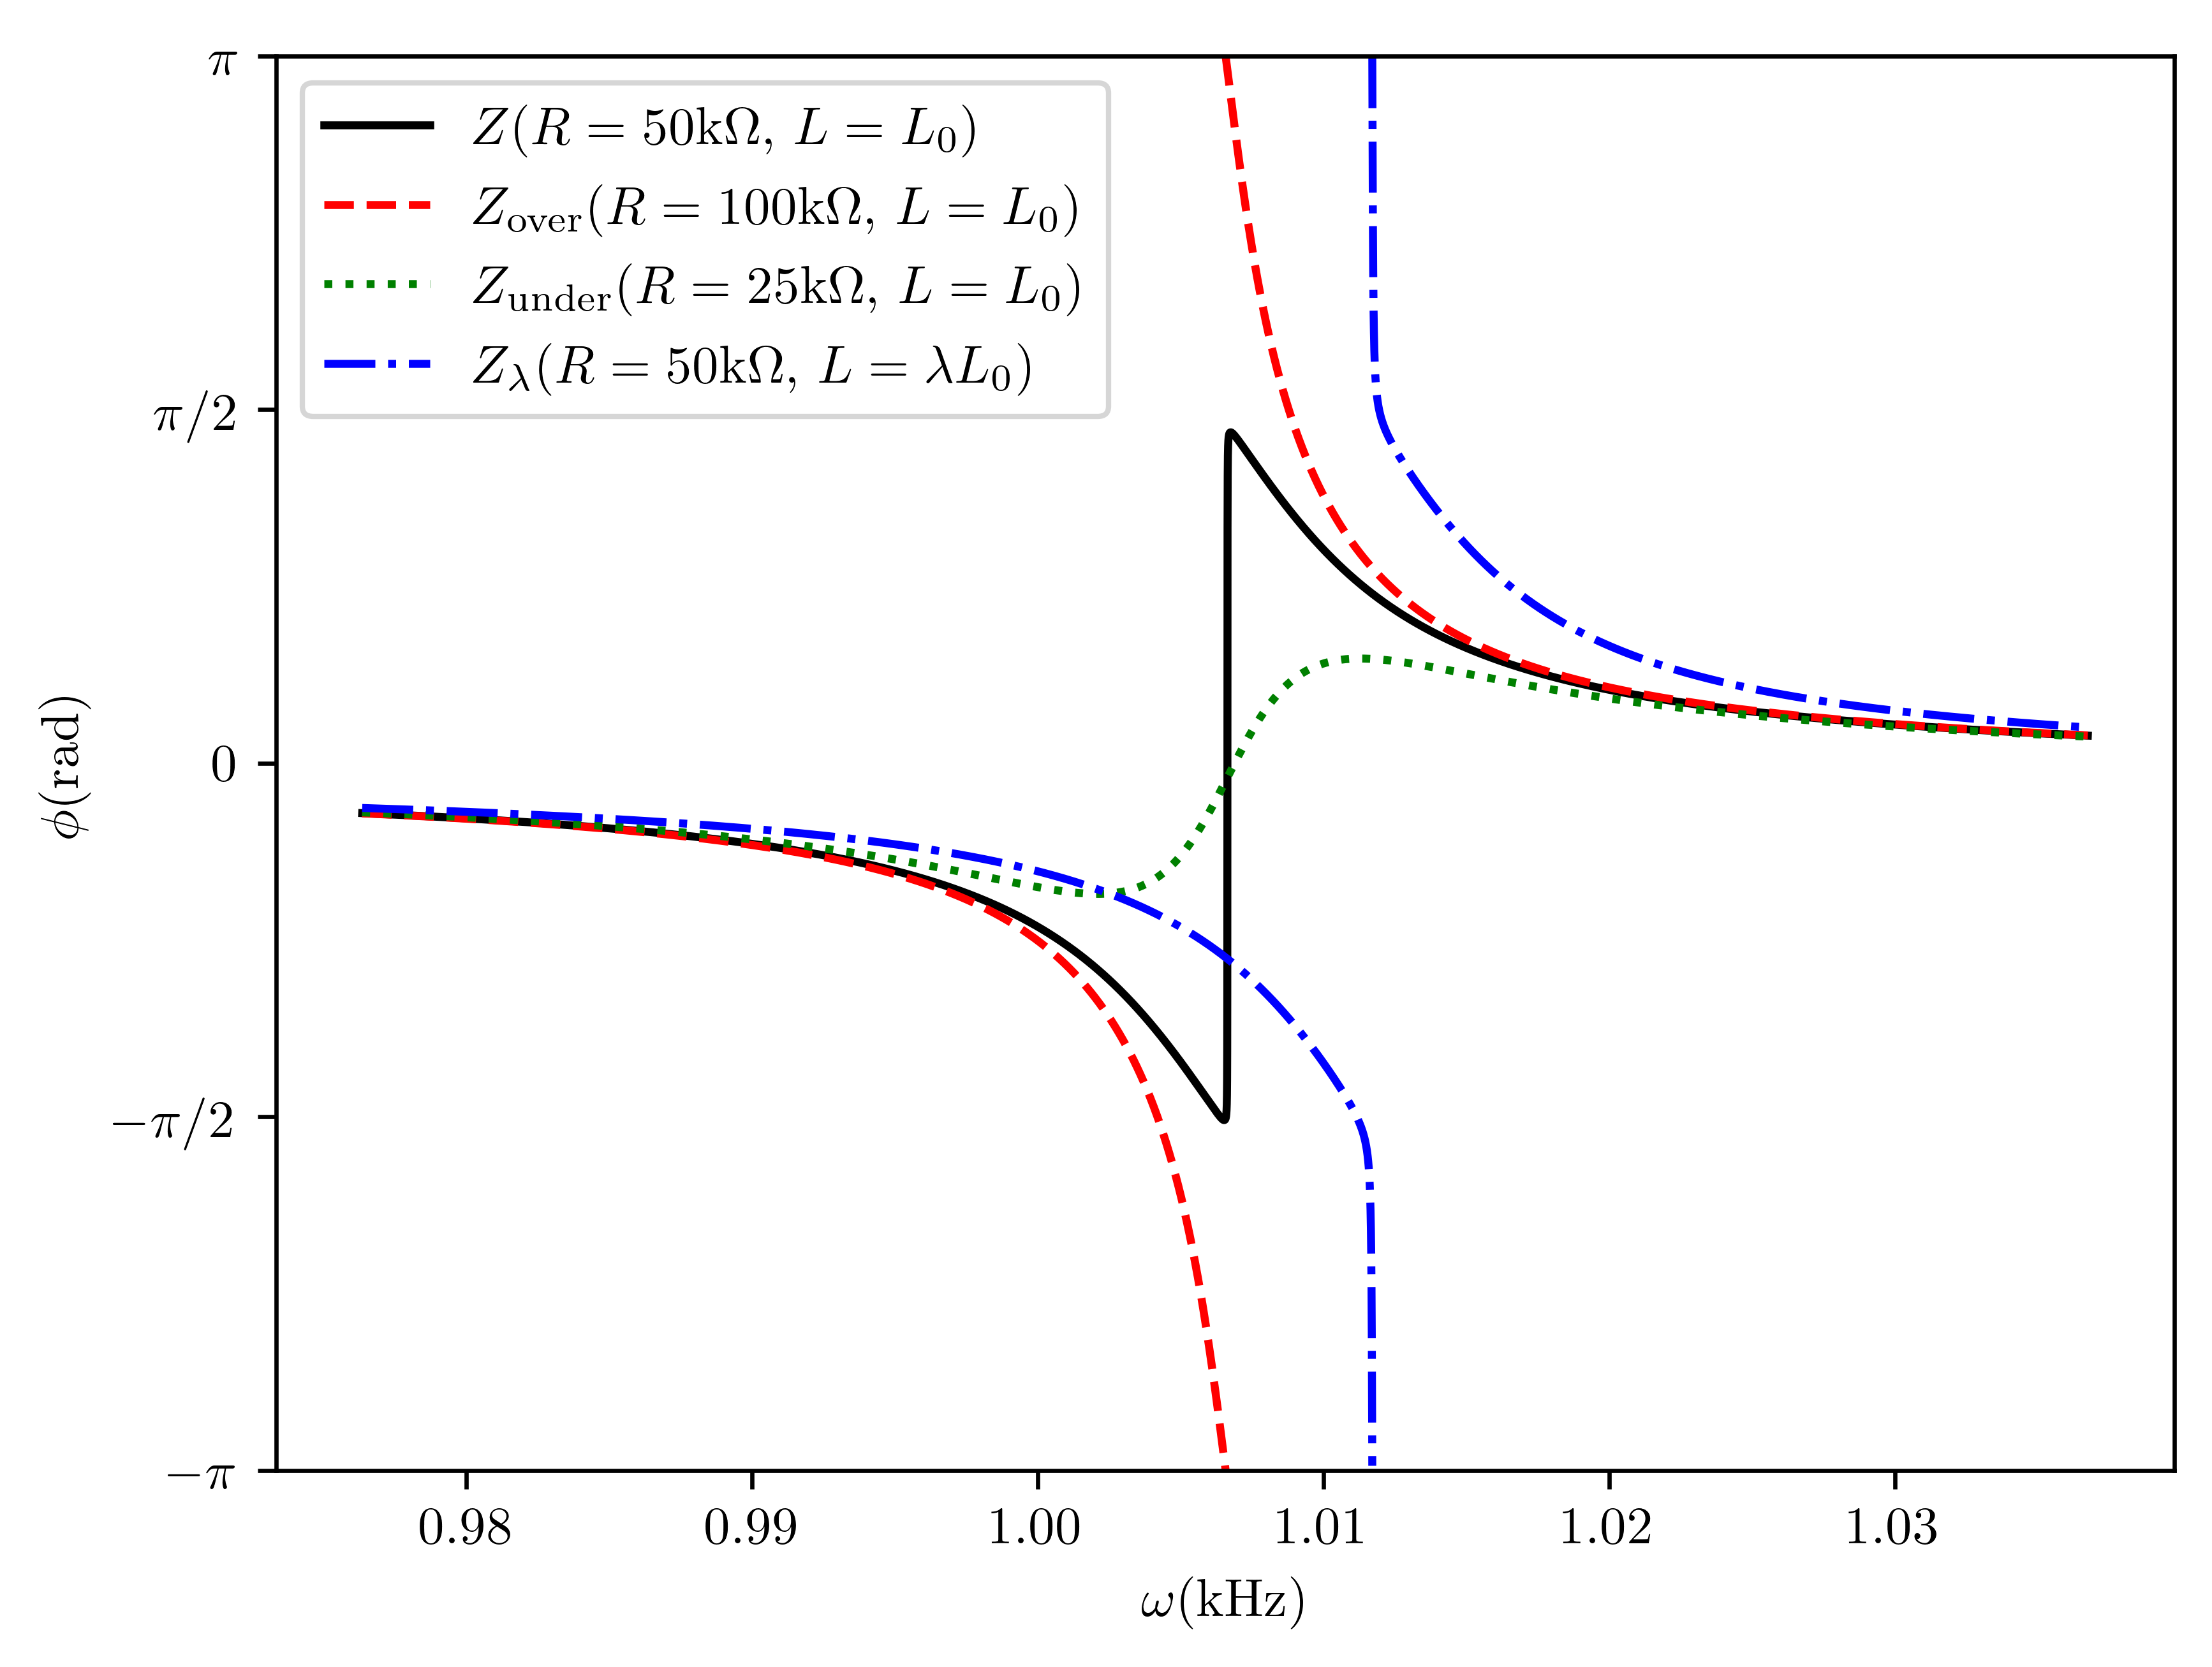
\includegraphics[width=\linewidth]{RLCParallel/ReflecPhase.png}
\end{subfigure}
\caption{Modulus and phase of \(\Gamma\) in multiple configurations}
\label{fig:ReflexCoeffAndPhase}
\end{figure}

In addition to this configuration, we have also graphed an over and an
under coupled system, and one with a slight variation of the inductance
(\(\lambda = 0.99\)).


\subsection{Contrast and it's optimization}
With an expression for the effective impedance of the system in resonance and
(more importantly) an expression for the resonant frequency, now we ask
ourselves the question: What are the values of \(L\) and \(C_{c}\) that
maximize the contrast
\(|\Delta\Gamma| = |\Gamma(\ROff) - \Gamma(\ROn)|\)?

Since on the lab the sizes of \(L\) and \(C_{p}\) are on the order of the ones used to
produce figure \ref{fig:ReflexCoeffAndPhase}, is easy to see that \(\omega_{r}\)
will be a lot more sensible to changes in \(L\) than to changes in \(C_{c}\),
and thus we will use \(C_{c}\) to optimize the contrast, while we will use \(L\)
to ensure that we stay in an acceptable frequency of operation.

With this in mind, we begin obtaining a workable expression of the contrast
by plugging expression \ref{eq:Wr} into \ref{eq:ImpParallel} without
considering any of the approximations related to \ref{eq:Wr}:

\begin{align}
\label{eq:ImpParallelResonant}
\begin{split}
    Z &= \frac{1}{j \omega C_{p} + \frac{1}{j \omega L} + \frac{1}{R}}
        + \frac{1}{j \omega C_{c}}\\
      &= \frac{  \omega R L}{R(1 - \omega^2 L C_{p}) + j \omega L}
        + \frac{1}{j \omega C_{c}}\\
      &= \frac{\frac{j R L}{\sqrt{L (C_{c} + C_{p})}}}{
          R\left(1 - \frac{\cancel{L} C_{p}}{\cancel{L}(C_{c} + C_{p})}\right)
            + \frac{j L}{\sqrt{L (C_{c} + C_{p})}}
            } + \frac{\sqrt{L (C_{c} + C_{p})}}{j C_{c}}\\
      &= \frac{j R L}{R\sqrt{L (C_{c} + C_{p})}
          \left(\frac{C_{c}}{C_{c} + C_{p}}\right) + j L}
          + \frac{\sqrt{L (C_{c} + C_{p})}}{j C_{c}}\\
      &= \frac{j R \cancel{L}}{R\frac{\cancel{L} \cancel{(C_{c} + C_{p})}}{
          \sqrt{L (C_{c} + C_{p})}}
          \left(\frac{C_{c}}{\cancel{C_{c} + C_{p}}}\right) + j \cancel{L}}
          + \frac{\sqrt{L (C_{c} + C_{p})}}{j C_{c}}\\
      &= \frac{j R}{RS + j} + \frac{1}{jS}
       = \frac{\cancel{-RS} + \cancel{RS} + j}{jRS^2 -S}
       = \frac{1}{RS^2 + jS}
       \text{ with } S = \frac{C_{c}}{\sqrt{L(C_{c} + C_{p})}}
\end{split}
\end{align}

Then we use this expression of the impedance to obtain the reflection coefficient,
but using the admittance of the transmission line instead of the impedance
(\(Y_{0} = 1/Z_{0}\))

\begin{align}
\begin{split}
    \Gamma &= \frac{Z - Z_{0}}{Z + Z_{0}} = \frac{Y_{0} - 1/Z}{Y_{0} + 1/Z}\\
           &= \frac{2Y_{0}}{Y_{0} + 1/Z} - 1 = \frac{2 Y_{0}}{RS^2 + Y_{0} + jS} - 1\\
           &= 2 Y_{0}\frac{RS^2 + Y_{0} - jS}{(RS^2 + Y_{0})^2 + S^2} - 1
\end{split}
\end{align}

Since \(\frac{1}{\sqrt{L (C_{c} + C_{p})}} \approx \omega_{r}\) then
\(\Im Z \approx 0\) and by extension \(\Im \Gamma \approx 0\), so

\begin{equation}
    \Gamma \approx 2 Y_{0}\frac{RS^2 + Y_{0}}{(RS^2 + Y_{0})^2 + S^2} - 1
\end{equation}

Next, using the parameters utilized for figure \ref{fig:ReflexCoeffAndPhase}
to get a sense of the scale, it is safe to assume that the following
approximation is correct

\begin{equation}
\label{eq:ParallelContrAprox}
    (RS^2 + Y_{0})^2 \gg S^2
\end{equation}

Which leaves us with the following expression for the reflection coefficient

\begin{equation}
\label{eq:ApproxReflecCoeff}
    \Gamma \approx \frac{2Y_{0}}{RS^2 + Y_{0}} - 1
\end{equation}

And this one for the contrast

\begin{equation}
\label{eq:ParallelContr}
    |\Delta\Gamma| = |\Gamma(R=\ROff) - \Gamma(R=\ROn)|
                   \approx 2Y_{0}\left|\frac{1}{
                   \ROff S^2 + Y_{0}} - \frac{1}{\ROn S^2 + Y_{0}
               }\right|
\end{equation}

Now, thanks to this simplified form of the contrast, to obtain the optimum
value for \(C_{c}\) we don't need any fancy tricks, just to derive with respect
to \(C_{c}\) and equate to \(0\). Doing this we arrive at the equation

\begin{equation}
\label{eq:ParallelContrOptS2NonRho}
    S^2 = \frac{Y_{0}}{\sqrt{\ROff\ROn}}
\end{equation}

And solving it for \(C_{c}\), we get the single solution
(for \(\ROn, \ROff, Y_{0}, L, C_{p}, C_{c} \geq 0\))

\begin{equation}
\label{eq:ParallelContrOptCcNonRho}
C_{c\text{Max}} = \frac{L Y_{0}}{2\sqrt{\ROff\ROn}}
\left(1 + \sqrt{1 + 4C_{p}\frac{\sqrt{\ROff\ROn}}{LY_{0}}}\right)
\end{equation}

We could simply plug this result into a simulation and call it a day, but with
a little bit more digging we can extract some interesting results.

First off, by the way the resistances appear in \ref{eq:ParallelContrOptS2NonRho}
and \ref{eq:ParallelContrOptCcNonRho} it leads really naturally to defining
a ratio parameter

\begin{equation}
\label{eq:RhoDef}
    \rho = \frac{\ROff}{\ROn}
\end{equation}

With it our expressions \ref{eq:ParallelContrOptS2NonRho} and
\ref{eq:ParallelContrOptCcNonRho} turn to

\begin{equation}
\label{eq:ParallelContrOptS2}
    S^2 = \frac{Y_{0}}{\sqrt{\rho}\ROn}
\end{equation}

\begin{equation}
\label{eq:ParallelContrOptCc}
C_{c\text{Max}} = \frac{L Y_{0}}{2\sqrt{\rho}\ROn}
\left(1 + \sqrt{1 + 4C_{p}\frac{\sqrt{\rho}\ROn}{LY_{0}}}\right)
\end{equation}

Then, by using the definition of \(S\) from \ref{eq:ImpParallelResonant} and
using impedance, we can rearrange \ref{eq:ParallelContrOptS2} to

\begin{equation}
\label{eq:ParallelTunning}
Z_{0} = \frac{L(C_{c}+C_{p})}{\sqrt{\rho}\ROn C_{c}^2}
\end{equation}

This might remind you of the expression \ref{eq:ApproximationZeff}, and it's
easy to see the parallelisms: In the previous case, given a resistance \(R\) we
can find a \(L\) and \(C_{c}\) (in the confines that the restrictions
\ref{eq:ApproxLWr}, \ref{eq:ApproxCcWr} and \ref{eq:ProtoZeffCond} allow)
that will make \ref{eq:ApproximationZeff} equal to \(Z_{0}\) and make \(\Gamma\)
equal to \(0\). For the contrast is the exact same, except that for that given
\(R\) it maximizes it instead of making it \(0\), and that we have 2 values
of \(R\), \(\ROn\) and \(\ROff = \rho \ROn\), so
which one do we use? Well it turns out that neither is the correct choice,
it is \(\sqrt{\ROff\ROn} = \sqrt{\rho}\ROn\),
the geometric mean of the resistances.

In addition to this insight, we can also use \ref{eq:ParallelContrOptS2} in
our approximation for the contrast (\ref{eq:ParallelContrAprox}) to see
that, when optimized, it only depends on the ratio of the resistances, and
that has a maximum value of 2, which is expected:

\begin{equation}
\label{eq:OptimumParallelContr}
    |\Delta\Gamma| \approx 2Y_{0}\left|\frac{1}{
                   \ROff S^2 + Y_{0}} - \frac{1}{\ROn S^2 + Y_{0}
               }\right|
                   = 2\left|
                   \frac{1}{\sqrt\rho + 1} - \frac{\sqrt\rho}{1 + \sqrt\rho}
                   \right|
                   = 2\left|
                   \frac{1 - \sqrt\rho}{1 + \sqrt\rho}
                   \right|
\end{equation}

After these results it seems appropriate to analyze with more detail the
approximations used, so we can contextualize the regime in which this works.
The first approximation done was \(\omega \approx \omega_{r}\), which boils
down to \ref{eq:ApproxLWr} and \ref{eq:ApproxCcWr}. The second approximation
was \ref{eq:ParallelContrAprox}, so let's see if with the optimum \(C_{c}\) it
holds. Using \ref{eq:ParallelContrOptS2} we have

\begin{equation}
    (RS^2 + Y_{0})^2 \gg S^2 \rightarrow
    \left(\frac{R Y_{0}}{\sqrt\rho \ROn} + Y_{0}\right)^2 \gg
    \frac{Y_{0}}{\sqrt\rho \ROn}
\end{equation}

Now, considering \(R = \ROn\) since it's the worst case scenario and
returning to the use of impedance instead of admittance, the condition turns to

\begin{equation}
\label{eq:ProtoOptParallelContrApprox}
    \left(\frac{1}{\sqrt\rho} + 1\right)^2 \gg
    \frac{Z_{0}}{\sqrt\rho \ROn}
\end{equation}

Since by definition \(\rho \leq 1\), we can take a stricter version for this
approximation but still achievable

\begin{equation}
\label{eq:OptParallelContrApprox}
    \ROn \gg Z_{0}
\end{equation}

This is clearly true in our case. In theory. Because you see, we've been
ignoring something up until now for the sake of simplicity, something that was
mentioned at the beginning of this section: the parasitic resistance \(R_{p}\).
As was said in the description of figure \ref{fig:RLC}, \(R_{p}\) is a virtual
resistance added in parallel with \(R_{text{SET}}\) to model losses in the
circuit, and it can make \(R < 50\unit{\kilo\ohm}\), so it is important that
we keep it in mind.

Thankfully is easy to add it back retroactively (that's why we've ignored it
up until now): we just need to do the following substitutions

\begin{align*}
    \ROn& \rightarrow R^{\prime}_{\text{On}}
    = \ROn \parallel R_{p}
    = \frac{\ROn R_{p}}{\ROn + R_{p}}\\
    \ROff& \rightarrow R^{\prime}_{\text{Off}}
    = \ROff \parallel R_{p}
    = \frac{\ROff R_{p}}{\ROff + R_{p}}\\
    \rho& \rightarrow \rho^{\prime} 
    = \frac{\ROff^{\prime}}{\ROn^{\prime}}
\end{align*}

If we give the same treatment to \(R_{p}\) as to \(\ROff\) by
introducing a ratio parameter

\begin{equation}
\label{eq:PiDef}
    \pi = \frac{R_{p}}{\ROn}
\end{equation}

Then the substitutions are

\begin{align*}
    \ROn& \rightarrow R^{\prime}_{\text{On}}
    = \frac{\pi}{1 + \pi} \ROn\\
    \ROff& \rightarrow R^{\prime}_{\text{Off}}
    = \frac{\rho\pi}{\rho + \pi}\ROn\\
    \rho& \rightarrow \rho^{\prime} 
    = \frac{\rho(1 + \pi)}{\rho + \pi}
\end{align*}

Taking this even further beyond with the fact that in an SET
\(\rho \approx \infty\) (in the Off state, no electrons are travelling through),
the substitutions are

\begin{align*}
    \ROn& \rightarrow R^{\prime}_{\text{On}}
    = \frac{\pi}{1 + \pi} \ROn\\
    \ROff& \rightarrow R^{\prime}_{\text{Off}}
    = \pi \ROn\\
    \rho& \rightarrow \rho^{\prime} 
    = 1 + \pi
\end{align*}

The introduction of the parasitic resistance and an infinite \(\ROff\)
doesn't change much, in the sense that for most of the expressions is better
to simply use the prime versions of \(\rho\) and \(\ROn\) for clarity.
Most. Because for two results in specific it helps: in
\ref{eq:OptimumParallelContr}

\begin{equation}
\label{eq:OptimumParallelContrOfPi}
    |\Delta\Gamma| \approx
                   2\left|
                   \frac{1 - \sqrt{1 + \pi}}{1 + \sqrt{1 + \pi}}
                   \right|
\end{equation}

And in \ref{eq:OptParallelContrApprox}

\begin{equation}
\label{eq:OptParallelContrApproxOfPi}
\frac{\pi}{1 + \pi}\ROn \gg Z_{0} \rightarrow
\pi \gg \frac{Z_{0}}{\ROn - Z_{0}}
\end{equation}

Using the values of \(Z_{0}\) and \(\ROn\) that we have been considering
up until now (\(50\unit{\ohm}\) and \(50\unit{\kilo\ohm}\) respectively) we can
see that for \ref{eq:OptParallelContrApprox} to work in a worse case scenario,
\(\pi\) must be a lot greater than \(10^{-3}\). It probably would
be, given that for a \(\pi\) 100 times greater,
\(|\Delta\Gamma| \approx 0.0477\), which isn't a good contrast to
aim for.

Finally, we check our results by comparing them against the numerically
calculated optimum contrast via a simulation that searches the optimum
value of \(C_{c}\) for a given value of \(\pi\).

\begin{figure}[t]
\centering
  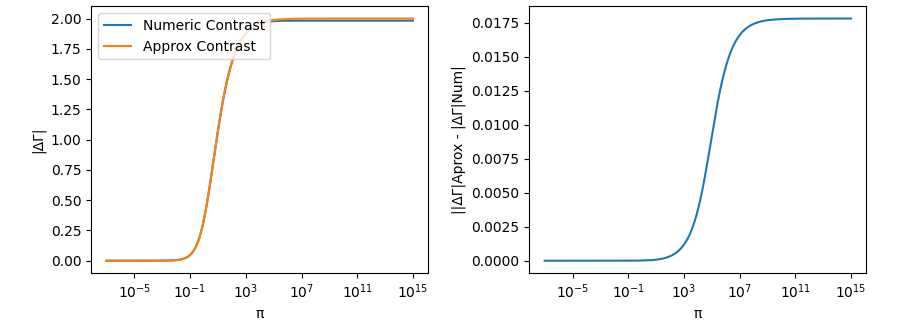
\includegraphics[width=\linewidth]{RLCParallel/OptContrComparison.png}
  \caption{Numerical optimum contrast and our formula (\ref{eq:OptimumParallelContrOfPi})
  with the difference between them.
\(L = 180\unit{\nano\henry}\), \(C_{p} = 500\unit{\femto\farad}\),
\(Z_{0} = 50\unit{\ohm}\), \(\ROn = 50\unit{\kilo\ohm}\),
\(\rho = 2\cdot10^{-6}\).}
\label{fig:ParallelContrComparison}
\end{figure}

As we can see in figure \ref{fig:ParallelContrComparison}, even though
the approximation gets worse for greater \(\pi\), it caps off to a difference of
\(0.0175\), which still makes it a pretty good approximation.

Next, we'll try to do the same analysis to a system with a variable inductance
via a kinetic inductor.

\end{document}
